\chapter{Related Work}

\section{2D and 3D Visualizations}

Although the focus of this thesis is on visualizing hierarchical networks in virtual reality, many concepts are the same or similar to its 2D or 3D counterparts. So first we want to give a brief overview of related 2D and 3D approaches in the field of network visualization.\\
Dynamic network visualization describes a research field where none or only few assumptions about the data are made, these techniques usually work by force-based layouts using node-link diagrams as we already summarized in the background section \ref{exp:force_based_background}. Furthermore, we want to discuss approaches dealing with hierarchical and multilayer structured datasets.

\subsection{Hierarchical Visualizations}

As we read in \ref{exp:tree} before, a preferred data structure to encode hierarchical information are trees.
Schulz \cite{schulz_treevisnet_2011} presented a good overview of different tree visualization techniques. A rough separation can be made by the representation of edges witch is either explicit or implicit. 

\subsubsection{Explicit approaches}
On explicit visualizations links are directly drawn as we have already seen in \ref{fig:simple_tree}. This core technique is used in numerous application domains and has been brought present over multiple scientific fields. Based on that concept researchers have developed many extensions.
LensTree \cite{song_lenstree_2006} for example, exchanges the axes and allows collapsing certain parts of the tree to display information structures like computer file directories. 
Armando et al. \cite{arce-orozco_radial_2017} uses radial instead of parallel axes to show the hierarchical relation, the root node is placed in the center and child nodes extend to all directions along the radius.
Munzer et al. \cite{munzner_h3_1997} extend the radial axis by a third dimension and displays the tree in the 3D hyperbolic space.
Robertson et al. \cite{robertson_cone_1991} also make use of the 3D space in his publications of the cone-tree and cam-tree, these display the child nodes as a circle below respectively beside their parents.  

\subsubsection{Implicit approaches - space filling}
The concept of nesting, which we also use in our layout, is heavenly used by space filling approaches. In addition, these usually encode the node-size into the used area as we have already seen in Figure \ref{fig:hierarchicalCirclePlot}.
Shneiderman \cite{shneiderman_tree_1992} presented this approach 1992 in the form of a tree map where he visualized the required disk space distribution of a file system. In addition to a common circle packing algorithm \ref{fig:hierarchicalCirclePlot}, Görtler \cite{gortler_bubble_2018} developed a bubble tree map technique which optimized the used space and allows encoding of additional properties via various shapes, draw strokes and colors. Sunburst charts are another common space filling technique to display node sizes in tree structures. 
As for 3D representations, Wang \cite{wang_visualization_2006} shows us a circular tree map extending to the z axis using cylinders. Instead of cylinders Balzer \cite{balzer_hierarchy_2004} uses nested hemispheres to visualize software structures.
Lastly, research is not limited to the layout of the visualization, as Itoh \cite{itoh_hierarchical_2004} shows us with their performance optimized technique for generating a rectangle packing tree map.

We can conclude that there are many approaches with various explicit and implicit layouts for tree visualizations, which focus on mapping hierarchical relationships for one network at a time. However, there are no links between multiple networks as this would mean there is a cycle in the original data and therefore breaking the definition of a tree structure in the first place. 

\subsection{Multilayer Visualization}
As we already figured out in section \ref{exp:multilayer}, the interesting part of multilayer visualizations is that it enables us to model relationships between multiple separated networks. Which was not possible with common node-link and tree visualization techniques we discussed before.\\
Domenico et al. \cite{de_domenico_muxviz_2015} presented their MuxVis Toolkit, an open-source software which is able to present multilayer datasets. In direct comparison to other approaches we have seen, this one stands out as it provides a complete and user-friendly software package with various layouts (see Figure \ref{fig:muxVisExample}) like a classical stacked one-line layer, a multi-line layer where multiple stacked layer planes are displayed beside each other, a force directed method and lastly a matrix layout. Besides these called 2.5D approaches we also see some classical 2D node-links networks, for example Ducruet \cite{ducruet_multilayer_nodate} display multiple networks of different marine traffic in a single graph just coded by color. 
A combination of multilevel graphs and hierarchical information can be seen in the approach by Eades \cite{eades_multilevel_1997} et al., here the authors group the nodes into nested clusters these are then displayed with a classical multilayer approach as flat layers below each other. The difference to general multilayer graphs is that each node has exact one connection to its (parent) node in the higher layer. 
Later on, Balzer et al. \cite{balzer_level--detail_2007} (see Figure \ref{fig:clusteredGraph}) created a similar visualization but instead of flat layers they used compact 3D surfaces to cluster and group their nodes. Their approach is really similar to ours as it also allows of nesting multiple levels of nodes and clusters, however they do not have a strict hierarchical aspect. 
Jonker et al. \cite{jonker_graph_2017} uses a level of detail approach where they group parts of the graph into clusters and only display single nodes when zooming into a specific tile. With their 2D layout therefore they achieve to visualize huge networks with a couple of hundred thousand nodes and links. 

\begin{figure}[h]
    \centering
    \begin{subfigure}[b]{0.75\columnwidth}
        \centering
        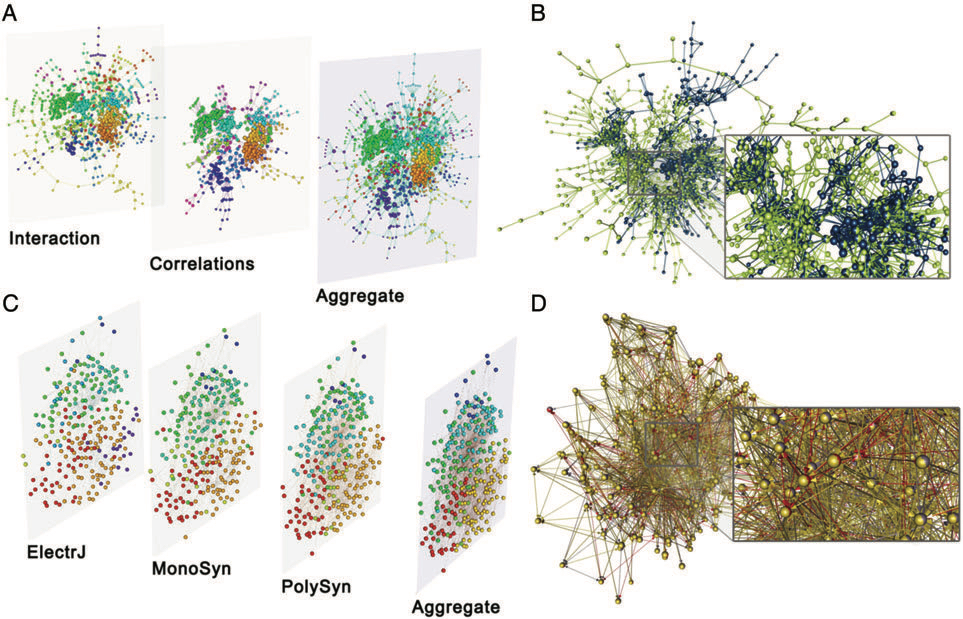
\includegraphics[width=\textwidth]{graphics/muxVisExample.jpg}
        \subcaption{Different supported layout techniques by MuxVis \cite{de_domenico_muxviz_2015}. }
        \label{fig:muxVisExample}
    \end{subfigure}
    \begin{subfigure}[b]{0.45\columnwidth}
        \centering
        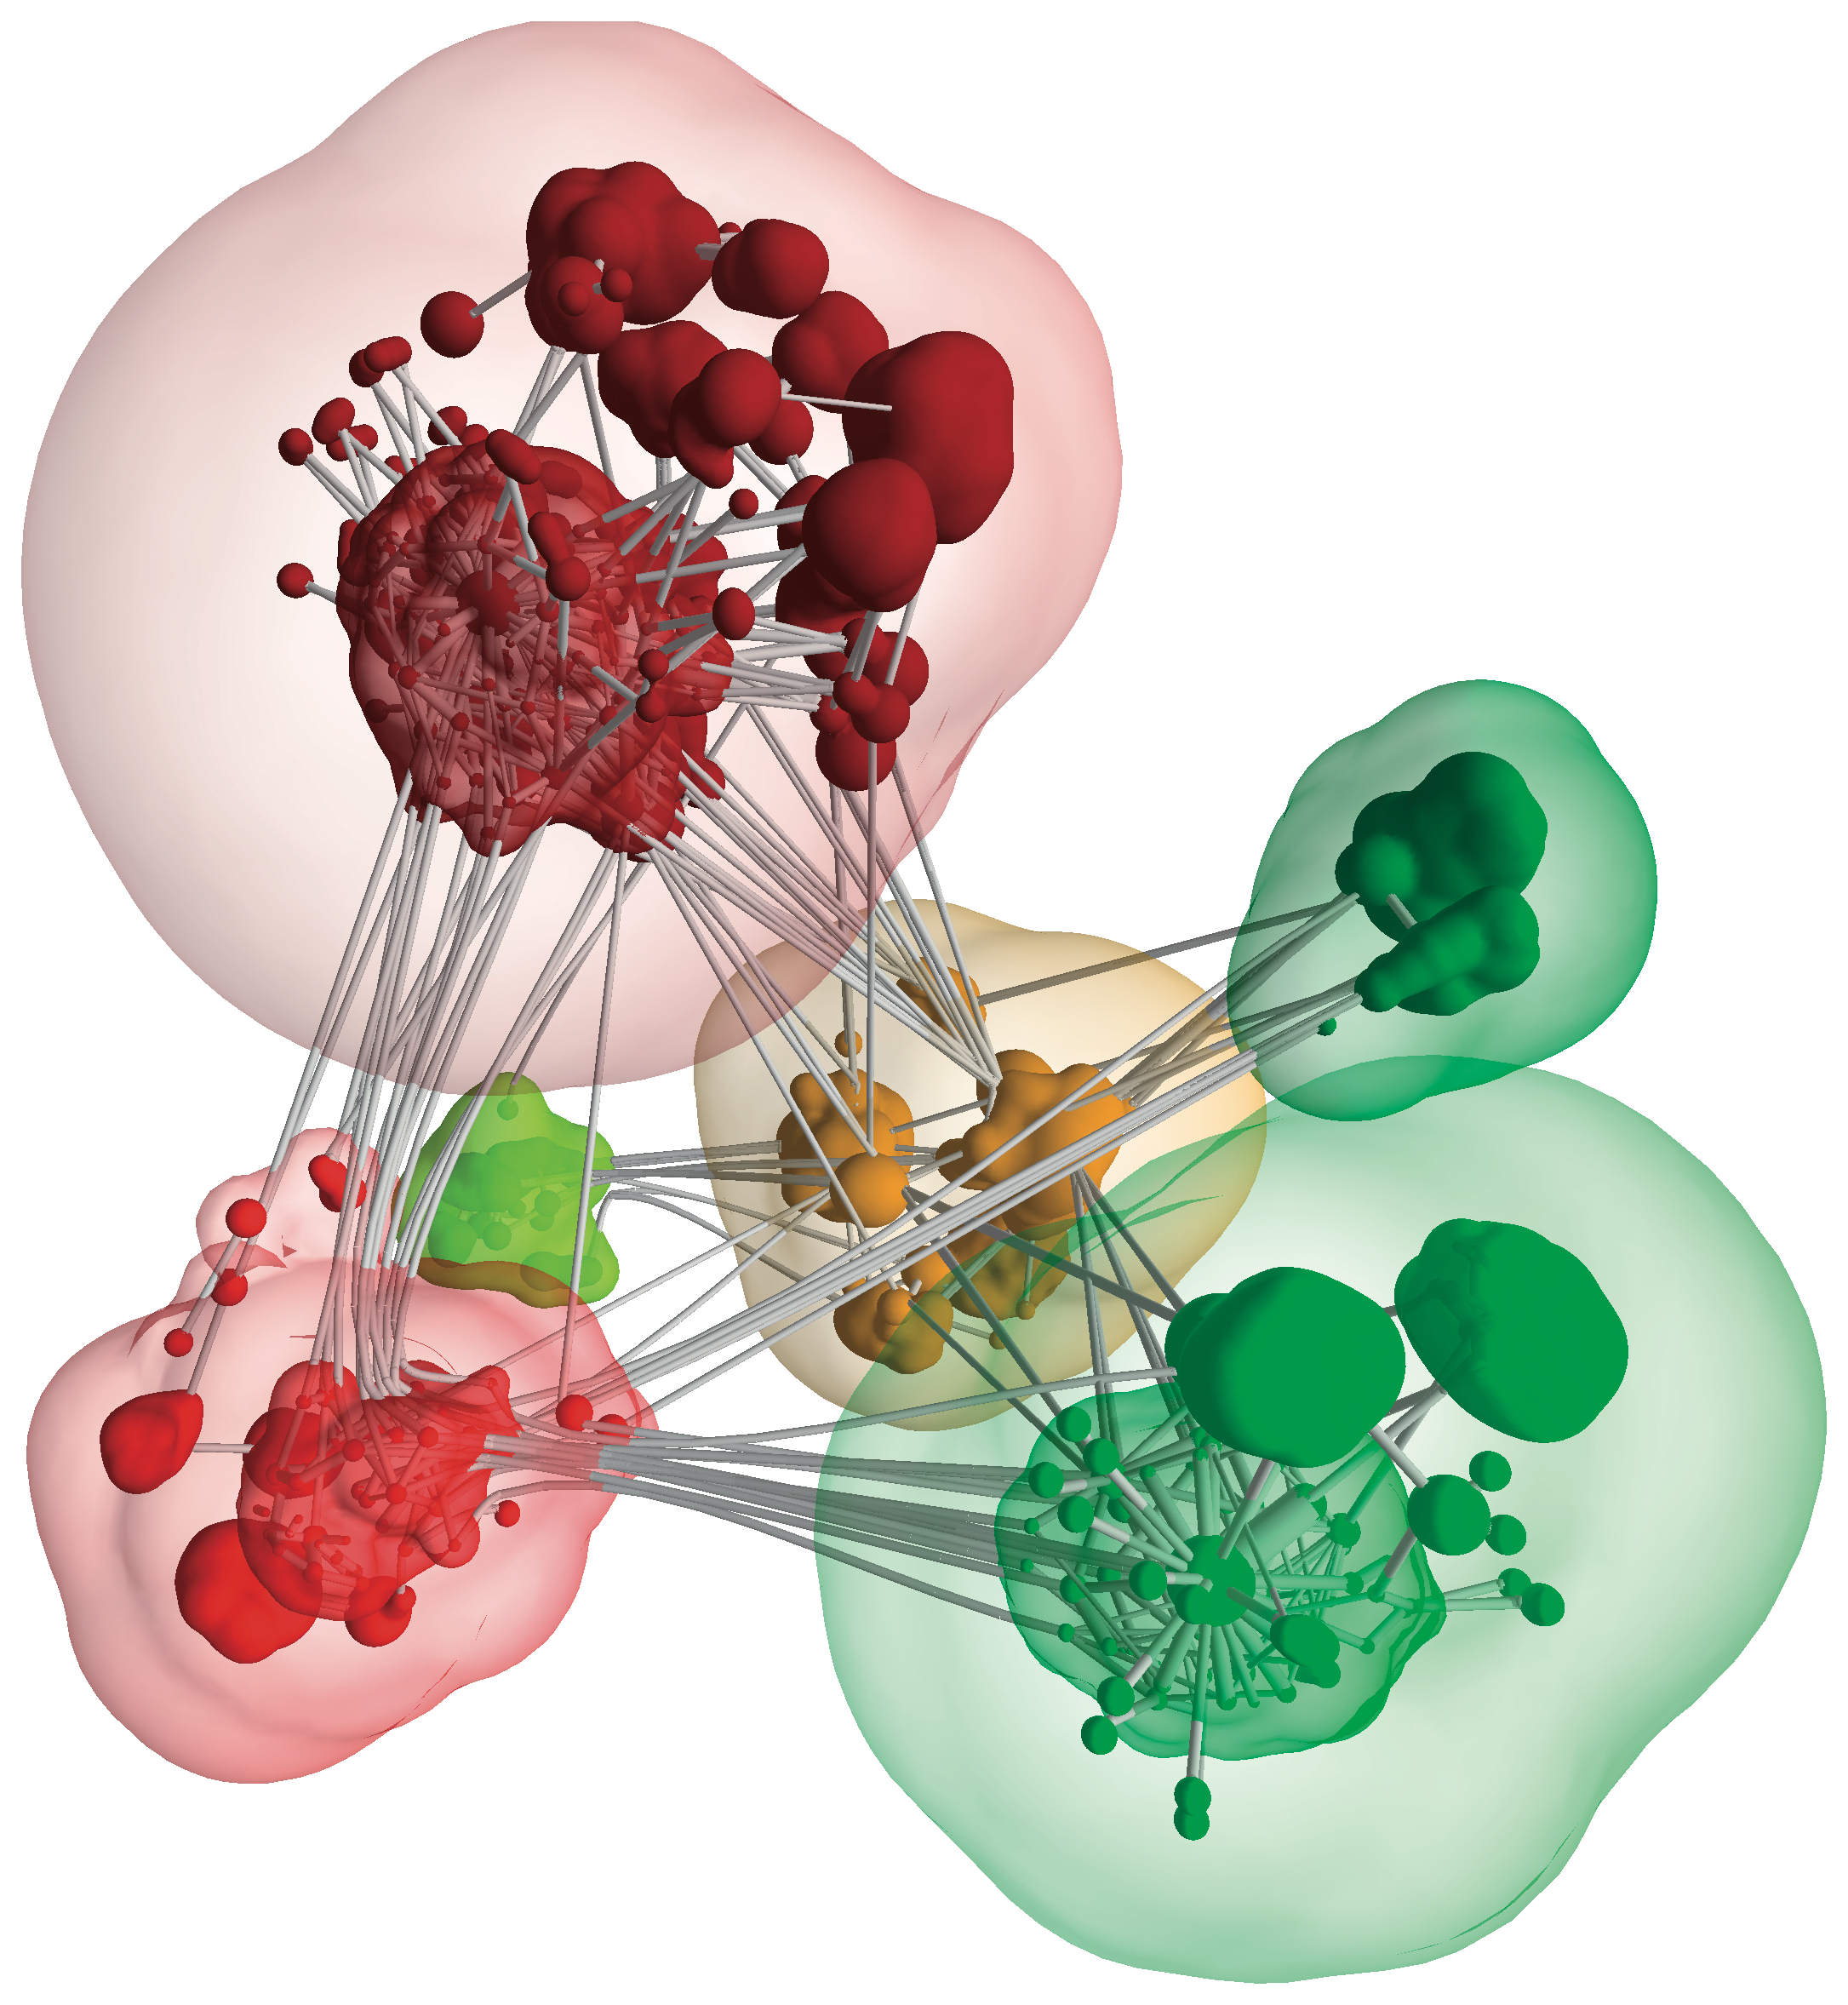
\includegraphics[width=\textwidth]{graphics/clusteredGraphVis.jpg}
        \subcaption{Visualization of a node-link dataset with multiple clusters from \cite{balzer_level--detail_2007}.}
        \label{fig:clusteredGraph}
    \end{subfigure}
    
    \caption[Optional caption for the figure list (often used to abbreviate long captions)]{Examples of multilayer visualizations.} % Remove the [...] argument if the original caption should be used in the figure list.
    \label{fig:relatedWorkExamples} 
  \end{figure}

\section{VR Visualizations}

\subsection{Layouts}

In VR, we see common 2D and 3D layout approaches like simple node-link diagrams adapted for the use in a 3D virtual scene. 
Some VR visualizations use a classical spring force layout to calculate their node positions \cite{drogemuller_examining_2020} \cite{sorger_immersive_2019}.
In other visualizations the position of the nodes comes directly from the data, for example Yang et al. \cite{yang_embodied_2020} use the t-SNE method \cite{maaten_visualizing_2008} to map the data attributes directly to x, y and z coordinates and display them as a point cloud scatter plot.
In addition to adapted layouts we also see some new ones specifically designed for the use in VR. Kwon et al. \cite{kwon_study_2016} presented a layout which displays all nodes on the surface of a sphere, the user stands inside the sphere and is therefore able to freely look around the visualization. Another approach comes from Halpin et al. \cite{halpin_exploring_2008} here the authors display the network on a flat 2D plane in front of the viewer, through interaction nodes can be extruded from the flat layout and highlighted on a separated layer.     

\subsection{Navigation}

The possibilities for navigation techniques in VR scenes, also called locomotion, heavenly depend on the target platform and experience the application is build for. As already describe in section \ref{exp:vr-experience}, there are seated-, standing- and room-scaled experiences depending on the used tracking technologies and available free play space.
At seated experiences the user is usually in front of a normal office desk setup while wearing the head mounted display. Therefore, real world movement is basically no option. 
Standing VR setups normally do not restrict movement, but the users available space to move is extremely limited. Rotating, leaning and hand movement should be no problem, but the application can not expect the user to walk around.
At room-scale VR setups the available space variate greatly, for example HTC Vive requires the user to have a minimum play space of $2m * 1.5m$ while a maximum (with 4 base stations) of $10m * 10m$ is possible. As a general rule of thumb we can say that for visualizations more available space is always better because the user can navigation through the scene just by walking. 
There are also some VR treadmills available which in theory provide infinite available space to walk, however we are not covering these are as they are pretty rare and expensive and therefore not suited for our purposes. The conclusion of a study by Usoh et al. \cite{usoh_walking_1999} emphasize the importance of walking inside a virtual scene, they found out that real walking provides a better immersive experience than virtual walking like a treadmill would provide and especially better than flying through the scene. 

In most scenarios however our virtual scene is bigger as the available space in the real world, therefore we need some techniques to navigate through the scene. For seated experiences Zielasko et al. \cite{zielasko_remain_2017} developed a method by using a virtual accelerator pedal tracked by a smartphone in the users pocket and another by leaning the head back and forth. These interactions are then are used to fly in the scene. Similar to the leaning approach Nguyen-Vo et al. \cite{nguyen-vo_simulated_2018} presented a technique which enables leaning with the chair while seated, to achieve that they simply used a swopper chair placed onto a Nintendo Wii Balance board which is able to track the direction of leaning by the distribution of weight.  
Drogemuller et al. \cite{drogemuller_examining_2020} summarized common navigation technique used by various VR applications. One of them is free flying using either gaze direction or the direction where the controller is pointed towards. Often free flying/walking is performed with the left controller while the right can be used for rotating the view without physical rotation, this is especially useful as users often interfere with the cable of the headset while rotating. Another use of the second controller is to describe a direction vector with both controllers for free flying, this is called two handed flying.\\
We can see many approaches use a free flying technique, however the problem is that many users especially these new to VR experience motion sickness in the context of VR also called cybersickness \cite{zielasko_remain_2017}.
To reduce the effect, a reduction of the field of view while flying with a smooth in and out transition is used by various papers and also often already implemented in common VR frameworks.\\
Beside flying teleportation is among the most used navigation techniques, usually the user can point at a location then press a button to teleport to that position.
This brings the advantage of reduced motion sickness because of the reduced animated movement. The challenge of teleportation is to select a point in three-dimensional space without any object nearby. While some approaches solve this with an adjustable teleport range, Lee et al. \cite{lee_evaluating_2020} presents a method to calculate the traveling distance based on the density of the area. In a parse environment with fewer objects nearby the distance is higher than in a dense environment with many objects.\\
Worlds-in-Miniature (WIM) \cite{drogemuller_examining_2020} takes the concept of a “minimap” from 2D visualizations into VR by displaying the entire graph in a small scale onto an object near the user, for example the top of the left or right controller. The user can move and rotate the miniature then select a point with the other controller which can be mapped to the position of the real graph and furthermore be used for various interaction possibilities like teleporting. Yang et al. \cite{yang_embodied_2020} shows us that locomotion can also be done via zooming and rotating. They use both controller to scale, rotate and translate the entire graph at the same time, similar to the zooming and panning used in touch screen applications. This allows the user to freely position the graph and therefore implicitly move around.

\subsection{Interaction}

Depending on the application context there are different goals for the interaction capabilities. For visualizations selection of details, filtering and brushing is important as we already summarized in the information seeking mantra \ref{seeking mantra} before. Therefore, researches have come up with different interaction techniques. The most basic approach would be an infinite ray cast selection based on the controller direction combined with a simple head up display or popup display the detail of the node or other selected entity. 
For filtering Drogemuller et al. \cite{drogemuller_vrige_2017} presented an interesting concept of a filter cube (see Figure \ref{fig:vrFilterCube}). The cube is mapped to an additional Vive tracker, the buttons and slider on it are used as a virtual input device activated via a virtual click on the button by a controller. 
The concept of a virtual toolbox or gadgets to interact with the environment however is not new, we already saw that in different VR games and creative applications for example Google Blocks VR or Tilt Brush by Google. Switching between multiple tools can be achieved by simply grabbing them with a controller or putting them back in their slot or bag.\\
In addition to the classical controller tracked interaction possibilities recent achievements in hand tracking technology make hand tracking without any additional equipment a reality as new VR headsets for example the Oculus Quest come with built in hand tracking. Besides built in technologies, there are also additional sensors available that can be attached to the VR headsets like the Leap Motion Controller. Yi-Jheng Huang et al. \cite{yi-jheng_huang_gesture_2017} used this sensor to build a complex hand gesture system especially designed for the manipulation of a node-link graph in VR, their gestures can be seen in Figure \ref{fig:vrHandGestures}. 

\begin{figure}[h]
    \centering
    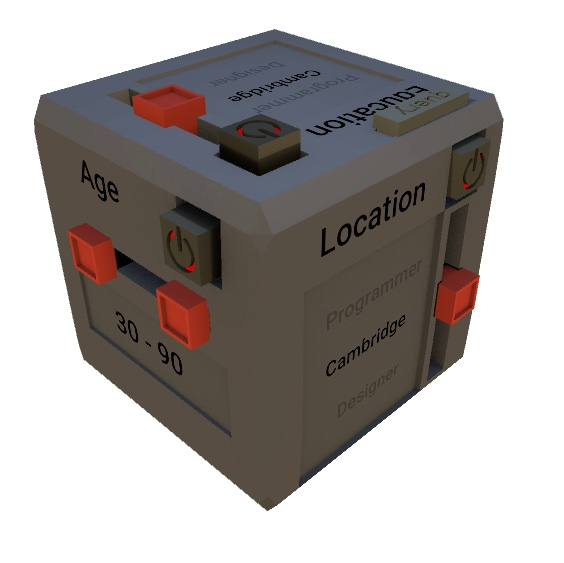
\includegraphics[width=0.4\textwidth]{graphics/filterCube.jpg}
    \caption{Filter cube of Drogemuller et al. \cite{drogemuller_vrige_2017}} 
    \label{fig:vrFilterCube} 
\end{figure}

\begin{figure}[h]
    \centering
    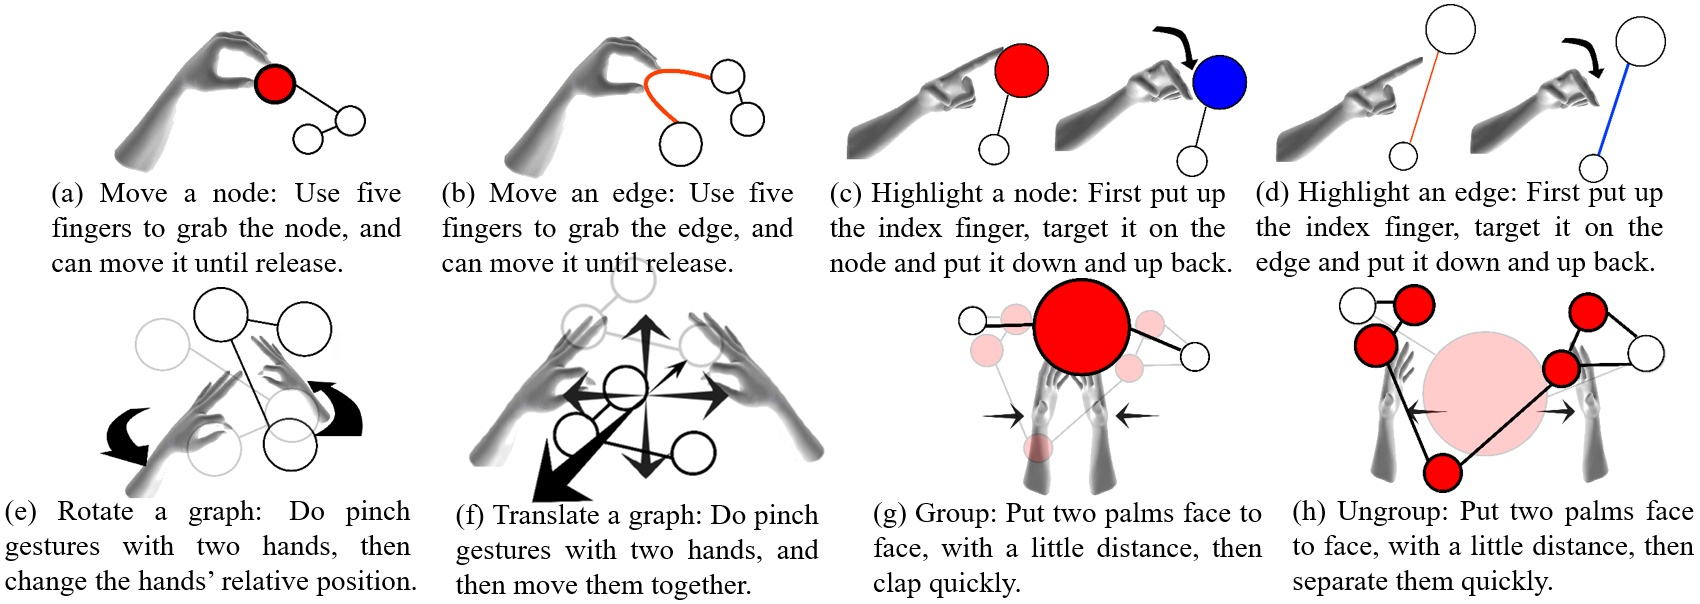
\includegraphics[width=1\textwidth]{graphics/handGestures.jpg}
    \caption{Different possibilities of hand gestures by Yi-Jheng Huang et al. \cite{yi-jheng_huang_gesture_2017}} 
    \label{fig:vrHandGestures} 
\end{figure}